\documentclass[1p]{elsarticle_modified}
%\bibliographystyle{elsarticle-num}

%\usepackage[colorlinks]{hyperref}
%\usepackage{abbrmath_seonhwa} %\Abb, \Ascr, \Acal ,\Abf, \Afrak
\usepackage{amsfonts}
\usepackage{amssymb}
\usepackage{amsmath}
\usepackage{amsthm}
\usepackage{scalefnt}
\usepackage{amsbsy}
\usepackage{kotex}
\usepackage{caption}
\usepackage{subfig}
\usepackage{color}
\usepackage{graphicx}
\usepackage{xcolor} %% white, black, red, green, blue, cyan, magenta, yellow
\usepackage{float}
\usepackage{setspace}
\usepackage{hyperref}

\usepackage{tikz}
\usetikzlibrary{arrows}

\usepackage{multirow}
\usepackage{array} % fixed length table
\usepackage{hhline}

%%%%%%%%%%%%%%%%%%%%%
\makeatletter
\renewcommand*\env@matrix[1][\arraystretch]{%
	\edef\arraystretch{#1}%
	\hskip -\arraycolsep
	\let\@ifnextchar\new@ifnextchar
	\array{*\c@MaxMatrixCols c}}
\makeatother %https://tex.stackexchange.com/questions/14071/how-can-i-increase-the-line-spacing-in-a-matrix
%%%%%%%%%%%%%%%

\usepackage[normalem]{ulem}

\newcommand{\msout}[1]{\ifmmode\text{\sout{\ensuremath{#1}}}\else\sout{#1}\fi}
%SOURCE: \msout is \stkout macro in https://tex.stackexchange.com/questions/20609/strikeout-in-math-mode

\newcommand{\cancel}[1]{
	\ifmmode
	{\color{red}\msout{#1}}
	\else
	{\color{red}\sout{#1}}
	\fi
}

\newcommand{\add}[1]{
	{\color{blue}\uwave{#1}}
}

\newcommand{\replace}[2]{
	\ifmmode
	{\color{red}\msout{#1}}{\color{blue}\uwave{#2}}
	\else
	{\color{red}\sout{#1}}{\color{blue}\uwave{#2}}
	\fi
}

\newcommand{\Sol}{\mathcal{S}} %segment
\newcommand{\D}{D} %diagram
\newcommand{\A}{\mathcal{A}} %arc


%%%%%%%%%%%%%%%%%%%%%%%%%%%%%5 test

\def\sl{\operatorname{\textup{SL}}(2,\Cbb)}
\def\psl{\operatorname{\textup{PSL}}(2,\Cbb)}
\def\quan{\mkern 1mu \triangleright \mkern 1mu}

\theoremstyle{definition}
\newtheorem{thm}{Theorem}[section]
\newtheorem{prop}[thm]{Proposition}
\newtheorem{lem}[thm]{Lemma}
\newtheorem{ques}[thm]{Question}
\newtheorem{cor}[thm]{Corollary}
\newtheorem{defn}[thm]{Definition}
\newtheorem{exam}[thm]{Example}
\newtheorem{rmk}[thm]{Remark}
\newtheorem{alg}[thm]{Algorithm}

\newcommand{\I}{\sqrt{-1}}
\begin{document}

%\begin{frontmatter}
%
%\title{Boundary parabolic representations of knots up to 8 crossings}
%
%%% Group authors per affiliation:
%\author{Yunhi Cho} 
%\address{Department of Mathematics, University of Seoul, Seoul, Korea}
%\ead{yhcho@uos.ac.kr}
%
%
%\author{Seonhwa Kim} %\fnref{s_kim}}
%\address{Center for Geometry and Physics, Institute for Basic Science, Pohang, 37673, Korea}
%\ead{ryeona17@ibs.re.kr}
%
%\author{Hyuk Kim}
%\address{Department of Mathematical Sciences, Seoul National University, Seoul 08826, Korea}
%\ead{hyukkim@snu.ac.kr}
%
%\author{Seokbeom Yoon}
%\address{Department of Mathematical Sciences, Seoul National University, Seoul, 08826,  Korea}
%\ead{sbyoon15@snu.ac.kr}
%
%\begin{abstract}
%We find all boundary parabolic representation of knots up to 8 crossings.
%
%\end{abstract}
%\begin{keyword}
%    \MSC[2010] 57M25 
%\end{keyword}
%
%\end{frontmatter}

%\linenumbers
%\tableofcontents
%
\newcommand\colored[1]{\textcolor{white}{\rule[-0.35ex]{0.8em}{1.4ex}}\kern-0.8em\color{red} #1}%
%\newcommand\colored[1]{\textcolor{white}{ #1}\kern-2.17ex	\textcolor{white}{ #1}\kern-1.81ex	\textcolor{white}{ #1}\kern-2.15ex\color{red}#1	}

{\Large $\underline{12n_{0831}~(K12n_{0831})}$}

\setlength{\tabcolsep}{10pt}
\renewcommand{\arraystretch}{1.6}
\vspace{1cm}\begin{tabular}{m{100pt}>{\centering\arraybackslash}m{274pt}}
\multirow{5}{120pt}{
	\centering
	\includegraphics[width=112pt]{../../../GIT/diagram.site/Diagrams/png/2920_12n_0831.png}\\
\ \ \ A knot diagram\footnotemark}&
\allowdisplaybreaks
\textbf{Linearized knot diagam} \\
\cline{2-2}
 &
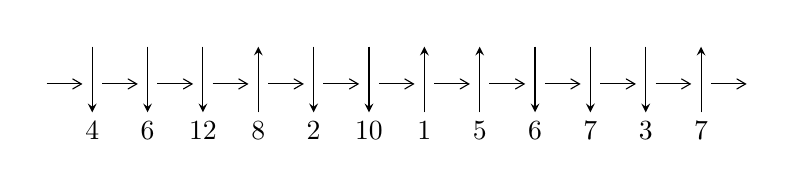
\begin{tikzpicture}[x=20pt, y=17pt]
	% nodes
	\node (C0) at (0, 0) {};
	\node (C1) at (1, 0) {};
	\node (C1U) at (1, +1) {};
	\node (C1D) at (1, -1) {4};

	\node (C2) at (2, 0) {};
	\node (C2U) at (2, +1) {};
	\node (C2D) at (2, -1) {6};

	\node (C3) at (3, 0) {};
	\node (C3U) at (3, +1) {};
	\node (C3D) at (3, -1) {12};

	\node (C4) at (4, 0) {};
	\node (C4U) at (4, +1) {};
	\node (C4D) at (4, -1) {8};

	\node (C5) at (5, 0) {};
	\node (C5U) at (5, +1) {};
	\node (C5D) at (5, -1) {2};

	\node (C6) at (6, 0) {};
	\node (C6U) at (6, +1) {};
	\node (C6D) at (6, -1) {10};

	\node (C7) at (7, 0) {};
	\node (C7U) at (7, +1) {};
	\node (C7D) at (7, -1) {1};

	\node (C8) at (8, 0) {};
	\node (C8U) at (8, +1) {};
	\node (C8D) at (8, -1) {5};

	\node (C9) at (9, 0) {};
	\node (C9U) at (9, +1) {};
	\node (C9D) at (9, -1) {6};

	\node (C10) at (10, 0) {};
	\node (C10U) at (10, +1) {};
	\node (C10D) at (10, -1) {7};

	\node (C11) at (11, 0) {};
	\node (C11U) at (11, +1) {};
	\node (C11D) at (11, -1) {3};

	\node (C12) at (12, 0) {};
	\node (C12U) at (12, +1) {};
	\node (C12D) at (12, -1) {7};
	\node (C13) at (13, 0) {};

	% arrows
	\draw[->,>={angle 60}]
	(C0) edge (C1) (C1) edge (C2) (C2) edge (C3) (C3) edge (C4) (C4) edge (C5) (C5) edge (C6) (C6) edge (C7) (C7) edge (C8) (C8) edge (C9) (C9) edge (C10) (C10) edge (C11) (C11) edge (C12) (C12) edge (C13) ;	\draw[->,>=stealth]
	(C1U) edge (C1D) (C2U) edge (C2D) (C3U) edge (C3D) (C4D) edge (C4U) (C5U) edge (C5D) (C6U) edge (C6D) (C7D) edge (C7U) (C8D) edge (C8U) (C9U) edge (C9D) (C10U) edge (C10D) (C11U) edge (C11D) (C12D) edge (C12U) ;
	\end{tikzpicture} \\
\hhline{~~} \\& 
\textbf{Solving Sequence} \\ \cline{2-2} 
 &
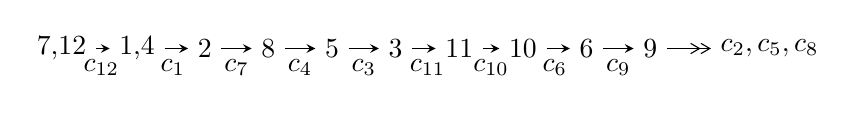
\begin{tikzpicture}[x=23pt, y=7pt]
	% node
	\node (A0) at (-1/8, 0) {7,12};
	\node (A1) at (17/16, 0) {1,4};
	\node (A2) at (17/8, 0) {2};
	\node (A3) at (25/8, 0) {8};
	\node (A4) at (33/8, 0) {5};
	\node (A5) at (41/8, 0) {3};
	\node (A6) at (49/8, 0) {11};
	\node (A7) at (57/8, 0) {10};
	\node (A8) at (65/8, 0) {6};
	\node (A9) at (73/8, 0) {9};
	\node (C1) at (1/2, -1) {$c_{12}$};
	\node (C2) at (13/8, -1) {$c_{1}$};
	\node (C3) at (21/8, -1) {$c_{7}$};
	\node (C4) at (29/8, -1) {$c_{4}$};
	\node (C5) at (37/8, -1) {$c_{3}$};
	\node (C6) at (45/8, -1) {$c_{11}$};
	\node (C7) at (53/8, -1) {$c_{10}$};
	\node (C8) at (61/8, -1) {$c_{6}$};
	\node (C9) at (69/8, -1) {$c_{9}$};
	\node (A10) at (11, 0) {$c_{2},c_{5},c_{8}$};

	% edge
	\draw[->,>=stealth]	
	(A0) edge (A1) (A1) edge (A2) (A2) edge (A3) (A3) edge (A4) (A4) edge (A5) (A5) edge (A6) (A6) edge (A7) (A7) edge (A8) (A8) edge (A9) ;
	\draw[->>,>={angle 60}]	
	(A9) edge (A10);
\end{tikzpicture} \\ 

\end{tabular} \\

\footnotetext{
The image of knot diagram is generated by the software ``\textbf{Draw programme}" developed by Andrew Bartholomew(\url{http://www.layer8.co.uk/maths/draw/index.htm\#Running-draw}), where we modified some parts for our purpose(\url{https://github.com/CATsTAILs/LinksPainter}).
}\phantom \\ \newline 
\centering \textbf{Ideals for irreducible components\footnotemark of $X_{\text{par}}$} 
 
\begin{align*}
I^u_{1}&=\langle 
-396999 u^{17}-586653 u^{16}+\cdots+343642 b-1550584,\\
\phantom{I^u_{1}}&\phantom{= \langle  }-523933 u^{17}-696379 u^{16}+\cdots+343642 a-2066672,\;u^{18}+u^{17}+\cdots+6 u-1\rangle \\
I^u_{2}&=\langle 
-3.98523\times10^{90} u^{43}+1.45733\times10^{90} u^{42}+\cdots+3.76570\times10^{90} b+3.66878\times10^{91},\\
\phantom{I^u_{2}}&\phantom{= \langle  }3.76232\times10^{91} u^{43}-6.44638\times10^{90} u^{42}+\cdots+5.27198\times10^{90} a-6.67170\times10^{92},\\
\phantom{I^u_{2}}&\phantom{= \langle  }2 u^{44}-29 u^{42}+\cdots-88 u-7\rangle \\
I^u_{3}&=\langle 
- u^5+u^4+2 u^3-3 u^2+2 b-4 u+4,\;- u^5+2 u^4+u^3-3 u^2+2 a-3 u+6,\\
\phantom{I^u_{3}}&\phantom{= \langle  }u^6-2 u^5- u^4+4 u^3+2 u^2-6 u+1\rangle \\
I^u_{4}&=\langle 
b-1,\;a+4 u-6,\;2 u^2-4 u+1\rangle \\
I^u_{5}&=\langle 
b-1,\;a^2-2,\;u+1\rangle \\
I^u_{6}&=\langle 
b- a+2,\;2 a^2-4 a+1,\;u+1\rangle \\
I^u_{7}&=\langle 
b-1,\;a,\;u-1\rangle \\
\\
\end{align*}
\raggedright * 7 irreducible components of $\dim_{\mathbb{C}}=0$, with total 75 representations.\\
\footnotetext{All coefficients of polynomials are rational numbers. But the coefficients are sometimes approximated in decimal forms when there is not enough margin.}
\newpage
\renewcommand{\arraystretch}{1}
\centering \section*{I. $I^u_{1}= \langle -3.97\times10^{5} u^{17}-5.87\times10^{5} u^{16}+\cdots+3.44\times10^{5} b-1.55\times10^{6},\;-5.24\times10^{5} u^{17}-6.96\times10^{5} u^{16}+\cdots+3.44\times10^{5} a-2.07\times10^{6},\;u^{18}+u^{17}+\cdots+6 u-1 \rangle$}
\flushleft \textbf{(i) Arc colorings}\\
\begin{tabular}{m{7pt} m{180pt} m{7pt} m{180pt} }
\flushright $a_{7}=$&$\begin{pmatrix}0\\u\end{pmatrix}$ \\
\flushright $a_{12}=$&$\begin{pmatrix}1\\0\end{pmatrix}$ \\
\flushright $a_{1}=$&$\begin{pmatrix}1\\- u^2\end{pmatrix}$ \\
\flushright $a_{4}=$&$\begin{pmatrix}1.52465 u^{17}+2.02647 u^{16}+\cdots-13.8141 u+6.01403\\1.15527 u^{17}+1.70716 u^{16}+\cdots-12.3278 u+4.51221\end{pmatrix}$ \\
\flushright $a_{2}=$&$\begin{pmatrix}-0.325219 u^{17}+0.133368 u^{16}+\cdots-5.76386 u+3.29663\\-1.39846 u^{17}-1.87149 u^{16}+\cdots+11.1270 u-3.17599\end{pmatrix}$ \\
\flushright $a_{8}=$&$\begin{pmatrix}u\\- u^3+u\end{pmatrix}$ \\
\flushright $a_{5}=$&$\begin{pmatrix}1.52465 u^{17}+2.02647 u^{16}+\cdots-13.8141 u+6.01403\\1.15527 u^{17}+1.70716 u^{16}+\cdots-12.3278 u+4.51221\end{pmatrix}$ \\
\flushright $a_{3}=$&$\begin{pmatrix}2.67992 u^{17}+3.73363 u^{16}+\cdots-26.1419 u+10.5262\\1.15527 u^{17}+1.70716 u^{16}+\cdots-12.3278 u+4.51221\end{pmatrix}$ \\
\flushright $a_{11}=$&$\begin{pmatrix}1.29270 u^{17}+1.81223 u^{16}+\cdots-10.6425 u+2.91863\\1.04950 u^{17}+1.64790 u^{16}+\cdots-11.8434 u+3.25485\end{pmatrix}$ \\
\flushright $a_{10}=$&$\begin{pmatrix}1.29270 u^{17}+1.81223 u^{16}+\cdots-10.6425 u+2.91863\\0.901071 u^{17}+1.31644 u^{16}+\cdots-10.0189 u+2.73532\end{pmatrix}$ \\
\flushright $a_{6}=$&$\begin{pmatrix}-1.44262 u^{17}-1.82416 u^{16}+\cdots+15.3771 u-4.47443\\-1.41888 u^{17}-1.96720 u^{16}+\cdots+13.3296 u-3.75667\end{pmatrix}$ \\
\flushright $a_{9}=$&$\begin{pmatrix}-0.501819 u^{17}-0.871197 u^{16}+\cdots+2.13386 u-1.52465\\-0.551894 u^{17}-0.465700 u^{16}+\cdots+1.41941 u-1.15527\end{pmatrix}$\\&\end{tabular}
\flushleft \textbf{(ii) Obstruction class $= -1$}\\~\\
\flushleft \textbf{(iii) Cusp Shapes $= -\frac{2646884}{171821} u^{17}-\frac{7468939}{343642} u^{16}+\cdots+\frac{54604739}{343642} u-\frac{10027319}{171821}$}\\~\\
\newpage\renewcommand{\arraystretch}{1}
\flushleft \textbf{(iv) u-Polynomials at the component}\newline \\
\begin{tabular}{m{50pt}|m{274pt}}
Crossings & \hspace{64pt}u-Polynomials at each crossing \\
\hline $$\begin{aligned}c_{1}\end{aligned}$$&$\begin{aligned}
&u^{18}-11 u^{17}+\cdots+160 u-32
\end{aligned}$\\
\hline $$\begin{aligned}c_{2},c_{3},c_{5}\\c_{11}\end{aligned}$$&$\begin{aligned}
&u^{18}- u^{17}+\cdots-3 u^3+1
\end{aligned}$\\
\hline $$\begin{aligned}c_{4},c_{7},c_{8}\\c_{12}\end{aligned}$$&$\begin{aligned}
&u^{18}- u^{17}+\cdots-6 u-1
\end{aligned}$\\
\hline $$\begin{aligned}c_{6},c_{9},c_{10}\end{aligned}$$&$\begin{aligned}
&u^{18}+10 u^{17}+\cdots-16 u+16
\end{aligned}$\\
\hline
\end{tabular}\\~\\
\newpage\renewcommand{\arraystretch}{1}
\flushleft \textbf{(v) Riley Polynomials at the component}\newline \\
\begin{tabular}{m{50pt}|m{274pt}}
Crossings & \hspace{64pt}Riley Polynomials at each crossing \\
\hline $$\begin{aligned}c_{1}\end{aligned}$$&$\begin{aligned}
&y^{18}-7 y^{17}+\cdots+3584 y+1024
\end{aligned}$\\
\hline $$\begin{aligned}c_{2},c_{3},c_{5}\\c_{11}\end{aligned}$$&$\begin{aligned}
&y^{18}-3 y^{17}+\cdots-14 y^2+1
\end{aligned}$\\
\hline $$\begin{aligned}c_{4},c_{7},c_{8}\\c_{12}\end{aligned}$$&$\begin{aligned}
&y^{18}-17 y^{17}+\cdots-28 y+1
\end{aligned}$\\
\hline $$\begin{aligned}c_{6},c_{9},c_{10}\end{aligned}$$&$\begin{aligned}
&y^{18}-8 y^{17}+\cdots-10880 y+256
\end{aligned}$\\
\hline
\end{tabular}\\~\\
\newpage\flushleft \textbf{(vi) Complex Volumes and Cusp Shapes}
$$\begin{array}{c|c|c}  
\text{Solutions to }I^u_{1}& \I (\text{vol} + \sqrt{-1}CS) & \text{Cusp shape}\\
 \hline 
\begin{aligned}
u &= \phantom{-}0.191738 + 1.076920 I \\
a &= \phantom{-}0.164769 - 0.216172 I \\
b &= -0.739470 - 0.526977 I\end{aligned}
 & -2.66808 - 4.00314 I & -9.75217 + 7.89932 I \\ \hline\begin{aligned}
u &= \phantom{-}0.191738 - 1.076920 I \\
a &= \phantom{-}0.164769 + 0.216172 I \\
b &= -0.739470 + 0.526977 I\end{aligned}
 & -2.66808 + 4.00314 I & -9.75217 - 7.89932 I \\ \hline\begin{aligned}
u &= \phantom{-}0.856890\phantom{ +0.000000I} \\
a &= \phantom{-}1.85099\phantom{ +0.000000I} \\
b &= -0.508119\phantom{ +0.000000I}\end{aligned}
 & -3.70252\phantom{ +0.000000I} & \phantom{-}0.540670\phantom{ +0.000000I} \\ \hline\begin{aligned}
u &= -1.268520 + 0.068652 I \\
a &= -0.20738 + 1.47520 I \\
b &= -1.13159 - 0.92777 I\end{aligned}
 & \phantom{-}6.81521 - 6.56774 I & -2.02682 + 4.35412 I \\ \hline\begin{aligned}
u &= -1.268520 - 0.068652 I \\
a &= -0.20738 - 1.47520 I \\
b &= -1.13159 + 0.92777 I\end{aligned}
 & \phantom{-}6.81521 + 6.56774 I & -2.02682 - 4.35412 I \\ \hline\begin{aligned}
u &= \phantom{-}0.099241 + 0.636465 I \\
a &= \phantom{-}0.938741 + 0.442143 I \\
b &= \phantom{-}0.365623 + 0.498306 I\end{aligned}
 & -0.56691 - 1.59781 I & -4.88738 + 2.87220 I \\ \hline\begin{aligned}
u &= \phantom{-}0.099241 - 0.636465 I \\
a &= \phantom{-}0.938741 - 0.442143 I \\
b &= \phantom{-}0.365623 - 0.498306 I\end{aligned}
 & -0.56691 + 1.59781 I & -4.88738 - 2.87220 I \\ \hline\begin{aligned}
u &= \phantom{-}1.384510 + 0.061181 I \\
a &= -0.025694 + 1.290750 I \\
b &= -0.757872 - 1.174240 I\end{aligned}
 & \phantom{-}9.74101 + 0.20067 I & \phantom{-}0.876554 + 0.056243 I \\ \hline\begin{aligned}
u &= \phantom{-}1.384510 - 0.061181 I \\
a &= -0.025694 - 1.290750 I \\
b &= -0.757872 + 1.174240 I\end{aligned}
 & \phantom{-}9.74101 - 0.20067 I & \phantom{-}0.876554 - 0.056243 I \\ \hline\begin{aligned}
u &= -0.598117\phantom{ +0.000000I} \\
a &= \phantom{-}2.91842\phantom{ +0.000000I} \\
b &= \phantom{-}0.874375\phantom{ +0.000000I}\end{aligned}
 & -6.04349\phantom{ +0.000000I} & -17.8030\phantom{ +0.000000I}\\
 \hline 
 \end{array}$$\newpage$$\begin{array}{c|c|c}  
\text{Solutions to }I^u_{1}& \I (\text{vol} + \sqrt{-1}CS) & \text{Cusp shape}\\
 \hline 
\begin{aligned}
u &= -1.36280 + 0.56912 I \\
a &= \phantom{-}0.123467 - 0.674233 I \\
b &= -0.019982 + 0.551107 I\end{aligned}
 & \phantom{-}2.28034 - 2.61810 I & -1.94443 - 3.90509 I \\ \hline\begin{aligned}
u &= -1.36280 - 0.56912 I \\
a &= \phantom{-}0.123467 + 0.674233 I \\
b &= -0.019982 - 0.551107 I\end{aligned}
 & \phantom{-}2.28034 + 2.61810 I & -1.94443 + 3.90509 I \\ \hline\begin{aligned}
u &= -1.53449 + 0.53389 I \\
a &= -0.200699 - 1.249540 I \\
b &= \phantom{-}1.26204 + 1.00770 I\end{aligned}
 & \phantom{-}6.5797 - 16.1278 I & -3.35911 + 8.29974 I \\ \hline\begin{aligned}
u &= -1.53449 - 0.53389 I \\
a &= -0.200699 + 1.249540 I \\
b &= \phantom{-}1.26204 - 1.00770 I\end{aligned}
 & \phantom{-}6.5797 + 16.1278 I & -3.35911 - 8.29974 I \\ \hline\begin{aligned}
u &= \phantom{-}1.56750 + 0.44100 I \\
a &= -0.207302 + 1.123790 I \\
b &= \phantom{-}0.815416 - 1.132280 I\end{aligned}
 & \phantom{-}9.08495 + 8.48084 I & -0.38289 - 5.34256 I \\ \hline\begin{aligned}
u &= \phantom{-}1.56750 - 0.44100 I \\
a &= -0.207302 - 1.123790 I \\
b &= \phantom{-}0.815416 + 1.132280 I\end{aligned}
 & \phantom{-}9.08495 - 8.48084 I & -0.38289 + 5.34256 I \\ \hline\begin{aligned}
u &= \phantom{-}0.348681\phantom{ +0.000000I} \\
a &= -0.719922\phantom{ +0.000000I} \\
b &= -1.63240\phantom{ +0.000000I}\end{aligned}
 & -10.4921\phantom{ +0.000000I} & \phantom{-}19.6160\phantom{ +0.000000I} \\ \hline\begin{aligned}
u &= \phantom{-}0.238190\phantom{ +0.000000I} \\
a &= \phantom{-}1.77872\phantom{ +0.000000I} \\
b &= \phantom{-}0.677803\phantom{ +0.000000I}\end{aligned}
 & -1.17090\phantom{ +0.000000I} & -9.40150\phantom{ +0.000000I}\\
 \hline 
 \end{array}$$\newpage\newpage\renewcommand{\arraystretch}{1}
\centering \section*{II. $I^u_{2}= \langle -3.99\times10^{90} u^{43}+1.46\times10^{90} u^{42}+\cdots+3.77\times10^{90} b+3.67\times10^{91},\;3.76\times10^{91} u^{43}-6.45\times10^{90} u^{42}+\cdots+5.27\times10^{90} a-6.67\times10^{92},\;2 u^{44}-29 u^{42}+\cdots-88 u-7 \rangle$}
\flushleft \textbf{(i) Arc colorings}\\
\begin{tabular}{m{7pt} m{180pt} m{7pt} m{180pt} }
\flushright $a_{7}=$&$\begin{pmatrix}0\\u\end{pmatrix}$ \\
\flushright $a_{12}=$&$\begin{pmatrix}1\\0\end{pmatrix}$ \\
\flushright $a_{1}=$&$\begin{pmatrix}1\\- u^2\end{pmatrix}$ \\
\flushright $a_{4}=$&$\begin{pmatrix}-7.13643 u^{43}+1.22276 u^{42}+\cdots+1065.91 u+126.550\\1.05830 u^{43}-0.387000 u^{42}+\cdots-112.988 u-9.74262\end{pmatrix}$ \\
\flushright $a_{2}=$&$\begin{pmatrix}0.806957 u^{43}-0.114485 u^{42}+\cdots-142.855 u-24.2057\\-0.107399 u^{43}-0.0284322 u^{42}+\cdots+28.3132 u+2.84251\end{pmatrix}$ \\
\flushright $a_{8}=$&$\begin{pmatrix}u\\- u^3+u\end{pmatrix}$ \\
\flushright $a_{5}=$&$\begin{pmatrix}-6.86544 u^{43}+1.11246 u^{42}+\cdots+1029.07 u+121.406\\1.23457 u^{43}-0.400196 u^{42}+\cdots-145.917 u-14.5004\end{pmatrix}$ \\
\flushright $a_{3}=$&$\begin{pmatrix}-6.07814 u^{43}+0.835762 u^{42}+\cdots+952.920 u+116.808\\1.05830 u^{43}-0.387000 u^{42}+\cdots-112.988 u-9.74262\end{pmatrix}$ \\
\flushright $a_{11}=$&$\begin{pmatrix}-1.21508 u^{43}+0.317864 u^{42}+\cdots+169.292 u+27.9292\\0.208421 u^{43}-0.0153784 u^{42}+\cdots-37.9937 u-4.00886\end{pmatrix}$ \\
\flushright $a_{10}=$&$\begin{pmatrix}-1.21508 u^{43}+0.317864 u^{42}+\cdots+169.292 u+27.9292\\0.326622 u^{43}-0.0913778 u^{42}+\cdots-47.7269 u-5.12139\end{pmatrix}$ \\
\flushright $a_{6}=$&$\begin{pmatrix}0.738865 u^{43}-0.0945014 u^{42}+\cdots-100.491 u-22.2900\\-0.0713589 u^{43}-0.0325985 u^{42}+\cdots+7.91982 u+0.387737\end{pmatrix}$ \\
\flushright $a_{9}=$&$\begin{pmatrix}-1.57557 u^{43}+0.540452 u^{42}+\cdots+85.6799 u+8.24586\\0.457009 u^{43}-0.0873987 u^{42}+\cdots-54.0595 u-7.38741\end{pmatrix}$\\&\end{tabular}
\flushleft \textbf{(ii) Obstruction class $= -1$}\\~\\
\flushleft \textbf{(iii) Cusp Shapes $= -1.66800 u^{43}+0.434075 u^{42}+\cdots+217.610 u+37.4599$}\\~\\
\newpage\renewcommand{\arraystretch}{1}
\flushleft \textbf{(iv) u-Polynomials at the component}\newline \\
\begin{tabular}{m{50pt}|m{274pt}}
Crossings & \hspace{64pt}u-Polynomials at each crossing \\
\hline $$\begin{aligned}c_{1}\end{aligned}$$&$\begin{aligned}
&(u^{22}+7 u^{21}+\cdots-6 u-2)^{2}
\end{aligned}$\\
\hline $$\begin{aligned}c_{2},c_{3},c_{5}\\c_{11}\end{aligned}$$&$\begin{aligned}
&2(2 u^{44}- u^{42}+\cdots-24 u+1)
\end{aligned}$\\
\hline $$\begin{aligned}c_{4},c_{7},c_{8}\\c_{12}\end{aligned}$$&$\begin{aligned}
&2(2 u^{44}-29 u^{42}+\cdots+88 u-7)
\end{aligned}$\\
\hline $$\begin{aligned}c_{6},c_{9},c_{10}\end{aligned}$$&$\begin{aligned}
&(u^{22}-4 u^{21}+\cdots+2 u-2)^{2}
\end{aligned}$\\
\hline
\end{tabular}\\~\\
\newpage\renewcommand{\arraystretch}{1}
\flushleft \textbf{(v) Riley Polynomials at the component}\newline \\
\begin{tabular}{m{50pt}|m{274pt}}
Crossings & \hspace{64pt}Riley Polynomials at each crossing \\
\hline $$\begin{aligned}c_{1}\end{aligned}$$&$\begin{aligned}
&(y^{22}+y^{21}+\cdots+48 y+4)^{2}
\end{aligned}$\\
\hline $$\begin{aligned}c_{2},c_{3},c_{5}\\c_{11}\end{aligned}$$&$\begin{aligned}
&4(4 y^{44}-4 y^{43}+\cdots-214 y+1)
\end{aligned}$\\
\hline $$\begin{aligned}c_{4},c_{7},c_{8}\\c_{12}\end{aligned}$$&$\begin{aligned}
&4(4 y^{44}-116 y^{43}+\cdots-4454 y+49)
\end{aligned}$\\
\hline $$\begin{aligned}c_{6},c_{9},c_{10}\end{aligned}$$&$\begin{aligned}
&(y^{22}-8 y^{21}+\cdots-40 y+4)^{2}
\end{aligned}$\\
\hline
\end{tabular}\\~\\
\newpage\flushleft \textbf{(vi) Complex Volumes and Cusp Shapes}
$$\begin{array}{c|c|c}  
\text{Solutions to }I^u_{2}& \I (\text{vol} + \sqrt{-1}CS) & \text{Cusp shape}\\
 \hline 
\begin{aligned}
u &= \phantom{-}1.00768\phantom{ +0.000000I} \\
a &= \phantom{-}0.540189\phantom{ +0.000000I} \\
b &= \phantom{-}1.30858\phantom{ +0.000000I}\end{aligned}
 & -3.29588\phantom{ +0.000000I} & -2.01200\phantom{ +0.000000I} \\ \hline\begin{aligned}
u &= -0.959621 + 0.038327 I \\
a &= \phantom{-}0.51386 + 2.68354 I \\
b &= -0.56442 - 2.02765 I\end{aligned}
 & \phantom{-}0.186770 + 0.086750 I & -6.26765 + 6.36021 I \\ \hline\begin{aligned}
u &= -0.959621 - 0.038327 I \\
a &= \phantom{-}0.51386 - 2.68354 I \\
b &= -0.56442 + 2.02765 I\end{aligned}
 & \phantom{-}0.186770 - 0.086750 I & -6.26765 - 6.36021 I \\ \hline\begin{aligned}
u &= \phantom{-}0.188755 + 0.896184 I \\
a &= \phantom{-}0.385957 - 0.105829 I \\
b &= \phantom{-}0.738143 + 0.476023 I\end{aligned}
 & -1.36349 - 1.79115 I & -8.68124 + 6.28577 I \\ \hline\begin{aligned}
u &= \phantom{-}0.188755 - 0.896184 I \\
a &= \phantom{-}0.385957 + 0.105829 I \\
b &= \phantom{-}0.738143 - 0.476023 I\end{aligned}
 & -1.36349 + 1.79115 I & -8.68124 - 6.28577 I \\ \hline\begin{aligned}
u &= \phantom{-}1.091200 + 0.395456 I \\
a &= \phantom{-}0.347759 + 0.568798 I \\
b &= \phantom{-}0.993160 - 0.453337 I\end{aligned}
 & -0.580514 + 1.104780 I & -4.00000 - 5.65044 I \\ \hline\begin{aligned}
u &= \phantom{-}1.091200 - 0.395456 I \\
a &= \phantom{-}0.347759 - 0.568798 I \\
b &= \phantom{-}0.993160 + 0.453337 I\end{aligned}
 & -0.580514 - 1.104780 I & -4.00000 + 5.65044 I \\ \hline\begin{aligned}
u &= -1.065490 + 0.625029 I \\
a &= -0.376962 + 1.132670 I \\
b &= -0.503539 - 0.055689 I\end{aligned}
 & \phantom{-}2.05974 - 7.04859 I & \phantom{-0.000000 } 0 \\ \hline\begin{aligned}
u &= -1.065490 - 0.625029 I \\
a &= -0.376962 - 1.132670 I \\
b &= -0.503539 + 0.055689 I\end{aligned}
 & \phantom{-}2.05974 + 7.04859 I & \phantom{-0.000000 } 0 \\ \hline\begin{aligned}
u &= -1.262810 + 0.021566 I \\
a &= -0.086610 + 1.327570 I \\
b &= \phantom{-}1.26751 - 0.99085 I\end{aligned}
 & \phantom{-}7.73724 - 0.72368 I & \phantom{-0.000000 } 0\\
 \hline 
 \end{array}$$\newpage$$\begin{array}{c|c|c}  
\text{Solutions to }I^u_{2}& \I (\text{vol} + \sqrt{-1}CS) & \text{Cusp shape}\\
 \hline 
\begin{aligned}
u &= -1.262810 - 0.021566 I \\
a &= -0.086610 - 1.327570 I \\
b &= \phantom{-}1.26751 + 0.99085 I\end{aligned}
 & \phantom{-}7.73724 + 0.72368 I & \phantom{-0.000000 } 0 \\ \hline\begin{aligned}
u &= \phantom{-}0.693940 + 0.232041 I \\
a &= \phantom{-}0.33396 - 1.93120 I \\
b &= -0.287053 + 0.030616 I\end{aligned}
 & -1.36349 + 1.79115 I & -8.68124 - 6.28577 I \\ \hline\begin{aligned}
u &= \phantom{-}0.693940 - 0.232041 I \\
a &= \phantom{-}0.33396 + 1.93120 I \\
b &= -0.287053 - 0.030616 I\end{aligned}
 & -1.36349 - 1.79115 I & -8.68124 + 6.28577 I \\ \hline\begin{aligned}
u &= -1.32704\phantom{ +0.000000I} \\
a &= \phantom{-}1.09776\phantom{ +0.000000I} \\
b &= -0.0760743\phantom{ +0.000000I}\end{aligned}
 & -3.29588\phantom{ +0.000000I} & \phantom{-0.000000 } 0 \\ \hline\begin{aligned}
u &= \phantom{-}1.221150 + 0.530023 I \\
a &= \phantom{-}0.017428 + 1.394390 I \\
b &= \phantom{-}1.08731 - 1.10905 I\end{aligned}
 & \phantom{-}0.55910 + 9.58499 I & \phantom{-0.000000 } 0 \\ \hline\begin{aligned}
u &= \phantom{-}1.221150 - 0.530023 I \\
a &= \phantom{-}0.017428 - 1.394390 I \\
b &= \phantom{-}1.08731 + 1.10905 I\end{aligned}
 & \phantom{-}0.55910 - 9.58499 I & \phantom{-0.000000 } 0 \\ \hline\begin{aligned}
u &= -1.212660 + 0.590602 I \\
a &= \phantom{-}0.240876 - 0.883836 I \\
b &= \phantom{-}0.312263 + 0.853014 I\end{aligned}
 & \phantom{-}1.85821 - 2.76391 I & \phantom{-0.000000 } 0 \\ \hline\begin{aligned}
u &= -1.212660 - 0.590602 I \\
a &= \phantom{-}0.240876 + 0.883836 I \\
b &= \phantom{-}0.312263 - 0.853014 I\end{aligned}
 & \phantom{-}1.85821 + 2.76391 I & \phantom{-0.000000 } 0 \\ \hline\begin{aligned}
u &= \phantom{-}1.343550 + 0.163045 I \\
a &= -0.18872 - 1.40724 I \\
b &= \phantom{-}0.75925 + 1.39471 I\end{aligned}
 & \phantom{-}8.21251 + 7.73197 I & \phantom{-0.000000 } 0 \\ \hline\begin{aligned}
u &= \phantom{-}1.343550 - 0.163045 I \\
a &= -0.18872 + 1.40724 I \\
b &= \phantom{-}0.75925 - 1.39471 I\end{aligned}
 & \phantom{-}8.21251 - 7.73197 I & \phantom{-0.000000 } 0\\
 \hline 
 \end{array}$$\newpage$$\begin{array}{c|c|c}  
\text{Solutions to }I^u_{2}& \I (\text{vol} + \sqrt{-1}CS) & \text{Cusp shape}\\
 \hline 
\begin{aligned}
u &= -0.884535 + 1.031500 I \\
a &= \phantom{-}0.227336 - 0.088919 I \\
b &= -0.457268 - 0.093641 I\end{aligned}
 & \phantom{-}1.85821 - 2.76391 I & \phantom{-0.000000 } 0 \\ \hline\begin{aligned}
u &= -0.884535 - 1.031500 I \\
a &= \phantom{-}0.227336 + 0.088919 I \\
b &= -0.457268 + 0.093641 I\end{aligned}
 & \phantom{-}1.85821 + 2.76391 I & \phantom{-0.000000 } 0 \\ \hline\begin{aligned}
u &= \phantom{-}1.271690 + 0.520977 I \\
a &= -0.16546 - 1.41673 I \\
b &= -0.930159 + 0.836061 I\end{aligned}
 & \phantom{-}2.05974 + 7.04859 I & \phantom{-0.000000 } 0 \\ \hline\begin{aligned}
u &= \phantom{-}1.271690 - 0.520977 I \\
a &= -0.16546 + 1.41673 I \\
b &= -0.930159 - 0.836061 I\end{aligned}
 & \phantom{-}2.05974 - 7.04859 I & \phantom{-0.000000 } 0 \\ \hline\begin{aligned}
u &= -0.613961 + 0.057476 I \\
a &= -0.959684 + 0.038453 I \\
b &= \phantom{-}1.217830 - 0.517219 I\end{aligned}
 & -0.580514 - 1.104780 I & -5.89293 + 5.65044 I \\ \hline\begin{aligned}
u &= -0.613961 - 0.057476 I \\
a &= -0.959684 - 0.038453 I \\
b &= \phantom{-}1.217830 + 0.517219 I\end{aligned}
 & -0.580514 + 1.104780 I & -5.89293 - 5.65044 I \\ \hline\begin{aligned}
u &= \phantom{-}1.346020 + 0.430624 I \\
a &= -0.093856 - 1.127210 I \\
b &= -1.105420 + 0.843659 I\end{aligned}
 & \phantom{-}3.25581 + 6.25880 I & \phantom{-0.000000 } 0 \\ \hline\begin{aligned}
u &= \phantom{-}1.346020 - 0.430624 I \\
a &= -0.093856 + 1.127210 I \\
b &= -1.105420 - 0.843659 I\end{aligned}
 & \phantom{-}3.25581 - 6.25880 I & \phantom{-0.000000 } 0 \\ \hline\begin{aligned}
u &= \phantom{-}0.45146 + 1.34717 I \\
a &= -0.0697853 - 0.0952976 I \\
b &= -0.924940 + 0.532455 I\end{aligned}
 & \phantom{-}0.55910 + 9.58499 I & \phantom{-0.000000 } 0 \\ \hline\begin{aligned}
u &= \phantom{-}0.45146 - 1.34717 I \\
a &= -0.0697853 + 0.0952976 I \\
b &= -0.924940 - 0.532455 I\end{aligned}
 & \phantom{-}0.55910 - 9.58499 I & \phantom{-0.000000 } 0\\
 \hline 
 \end{array}$$\newpage$$\begin{array}{c|c|c}  
\text{Solutions to }I^u_{2}& \I (\text{vol} + \sqrt{-1}CS) & \text{Cusp shape}\\
 \hline 
\begin{aligned}
u &= -1.42044 + 0.15034 I \\
a &= \phantom{-}0.185356 + 0.976083 I \\
b &= -0.751350 - 0.962354 I\end{aligned}
 & \phantom{-}4.35834 - 0.41728 I & \phantom{-0.000000 } 0 \\ \hline\begin{aligned}
u &= -1.42044 - 0.15034 I \\
a &= \phantom{-}0.185356 - 0.976083 I \\
b &= -0.751350 + 0.962354 I\end{aligned}
 & \phantom{-}4.35834 + 0.41728 I & \phantom{-0.000000 } 0 \\ \hline\begin{aligned}
u &= \phantom{-}1.46909\phantom{ +0.000000I} \\
a &= -0.934519\phantom{ +0.000000I} \\
b &= \phantom{-}0.929346\phantom{ +0.000000I}\end{aligned}
 & -6.50325\phantom{ +0.000000I} & \phantom{-0.000000 } 0 \\ \hline\begin{aligned}
u &= \phantom{-}1.62269 + 0.27689 I \\
a &= \phantom{-}0.443344 - 1.014190 I \\
b &= -0.843009 + 1.064050 I\end{aligned}
 & \phantom{-}7.73724 + 0.72368 I & \phantom{-0.000000 } 0 \\ \hline\begin{aligned}
u &= \phantom{-}1.62269 - 0.27689 I \\
a &= \phantom{-}0.443344 + 1.014190 I \\
b &= -0.843009 - 1.064050 I\end{aligned}
 & \phantom{-}7.73724 - 0.72368 I & \phantom{-0.000000 } 0 \\ \hline\begin{aligned}
u &= -1.61575 + 0.49113 I \\
a &= \phantom{-}0.250844 + 1.051830 I \\
b &= -1.22355 - 0.90329 I\end{aligned}
 & \phantom{-}8.21251 - 7.73197 I & \phantom{-0.000000 } 0 \\ \hline\begin{aligned}
u &= -1.61575 - 0.49113 I \\
a &= \phantom{-}0.250844 - 1.051830 I \\
b &= -1.22355 + 0.90329 I\end{aligned}
 & \phantom{-}8.21251 + 7.73197 I & \phantom{-0.000000 } 0 \\ \hline\begin{aligned}
u &= -0.223680 + 0.077265 I \\
a &= \phantom{-}5.50128 + 1.65439 I \\
b &= -0.264264 - 0.788553 I\end{aligned}
 & \phantom{-}4.35834 + 0.41728 I & \phantom{-}1.220508 + 0.567857 I \\ \hline\begin{aligned}
u &= -0.223680 - 0.077265 I \\
a &= \phantom{-}5.50128 - 1.65439 I \\
b &= -0.264264 + 0.788553 I\end{aligned}
 & \phantom{-}4.35834 - 0.41728 I & \phantom{-}1.220508 - 0.567857 I \\ \hline\begin{aligned}
u &= \phantom{-}0.224841\phantom{ +0.000000I} \\
a &= \phantom{-}5.44634\phantom{ +0.000000I} \\
b &= -1.36290\phantom{ +0.000000I}\end{aligned}
 & -6.50325\phantom{ +0.000000I} & -14.7860\phantom{ +0.000000I}\\
 \hline 
 \end{array}$$\newpage$$\begin{array}{c|c|c}  
\text{Solutions to }I^u_{2}& \I (\text{vol} + \sqrt{-1}CS) & \text{Cusp shape}\\
 \hline 
\begin{aligned}
u &= -0.179416 + 0.100194 I \\
a &= -6.69182 - 0.26567 I \\
b &= \phantom{-}0.206450 + 0.863665 I\end{aligned}
 & \phantom{-}3.25581 - 6.25880 I & -1.71216 + 4.44144 I \\ \hline\begin{aligned}
u &= -0.179416 - 0.100194 I \\
a &= -6.69182 + 0.26567 I \\
b &= \phantom{-}0.206450 - 0.863665 I\end{aligned}
 & \phantom{-}3.25581 + 6.25880 I & -1.71216 - 4.44144 I \\ \hline\begin{aligned}
u &= -0.47940 + 2.17394 I \\
a &= \phantom{-}0.181439 + 0.022852 I \\
b &= \phantom{-}0.873580 + 0.079126 I\end{aligned}
 & \phantom{-}0.186770 - 0.086750 I & \phantom{-0.000000 } 0 \\ \hline\begin{aligned}
u &= -0.47940 - 2.17394 I \\
a &= \phantom{-}0.181439 - 0.022852 I \\
b &= \phantom{-}0.873580 - 0.079126 I\end{aligned}
 & \phantom{-}0.186770 + 0.086750 I & \phantom{-0.000000 } 0\\
 \hline 
 \end{array}$$\newpage\newpage\renewcommand{\arraystretch}{1}
\centering \section*{III. $I^u_{3}= \langle - u^5+u^4+2 u^3-3 u^2+2 b-4 u+4,\;- u^5+2 u^4+u^3-3 u^2+2 a-3 u+6,\;u^6-2 u^5- u^4+4 u^3+2 u^2-6 u+1 \rangle$}
\flushleft \textbf{(i) Arc colorings}\\
\begin{tabular}{m{7pt} m{180pt} m{7pt} m{180pt} }
\flushright $a_{7}=$&$\begin{pmatrix}0\\u\end{pmatrix}$ \\
\flushright $a_{12}=$&$\begin{pmatrix}1\\0\end{pmatrix}$ \\
\flushright $a_{1}=$&$\begin{pmatrix}1\\- u^2\end{pmatrix}$ \\
\flushright $a_{4}=$&$\begin{pmatrix}\frac{1}{2} u^5- u^4+\cdots+\frac{3}{2} u-3\\\frac{1}{2} u^5-\frac{1}{2} u^4- u^3+\frac{3}{2} u^2+2 u-2\end{pmatrix}$ \\
\flushright $a_{2}=$&$\begin{pmatrix}- u^5+2 u^4+u^3-4 u^2-2 u+6\\-\frac{1}{2} u^5+u^4+\cdots-\frac{3}{2} u+3\end{pmatrix}$ \\
\flushright $a_{8}=$&$\begin{pmatrix}u\\- u^3+u\end{pmatrix}$ \\
\flushright $a_{5}=$&$\begin{pmatrix}\frac{1}{2} u^5- u^4+\cdots+\frac{3}{2} u-3\\\frac{1}{2} u^5-\frac{3}{2} u^4- u^3+\frac{5}{2} u^2+2 u-2\end{pmatrix}$ \\
\flushright $a_{3}=$&$\begin{pmatrix}u^5-\frac{3}{2} u^4-\frac{3}{2} u^3+3 u^2+\frac{7}{2} u-5\\\frac{1}{2} u^5-\frac{1}{2} u^4- u^3+\frac{3}{2} u^2+2 u-2\end{pmatrix}$ \\
\flushright $a_{11}=$&$\begin{pmatrix}u^5-2 u^4-\frac{3}{2} u^3+\frac{9}{2} u^2+3 u-\frac{13}{2}\\-\frac{1}{2} u^4+\frac{3}{2} u^2-\frac{1}{2} u-\frac{5}{2}\end{pmatrix}$ \\
\flushright $a_{10}=$&$\begin{pmatrix}u^5-2 u^4-\frac{3}{2} u^3+\frac{9}{2} u^2+3 u-\frac{13}{2}\\\frac{1}{2} u^5- u^4- u^3+2 u^2+\frac{1}{2} u-\frac{5}{2}\end{pmatrix}$ \\
\flushright $a_{6}=$&$\begin{pmatrix}-\frac{3}{2} u^5+\frac{5}{2} u^4+2 u^3-\frac{9}{2} u^2-4 u+7\\-\frac{1}{2} u^3-\frac{1}{2} u^2+u+\frac{5}{2}\end{pmatrix}$ \\
\flushright $a_{9}=$&$\begin{pmatrix}-\frac{1}{2} u^3-\frac{1}{2} u^2+u+\frac{1}{2}\\\frac{1}{2} u^5+\frac{1}{2} u^4-\frac{3}{2} u^3- u^2+\frac{1}{2}\end{pmatrix}$\\&\end{tabular}
\flushleft \textbf{(ii) Obstruction class $= 1$}\\~\\
\flushleft \textbf{(iii) Cusp Shapes $= \frac{17}{2} u^5-16 u^4-12 u^3+27 u^2+\frac{55}{2} u-\frac{81}{2}$}\\~\\
\newpage\renewcommand{\arraystretch}{1}
\flushleft \textbf{(iv) u-Polynomials at the component}\newline \\
\begin{tabular}{m{50pt}|m{274pt}}
Crossings & \hspace{64pt}u-Polynomials at each crossing \\
\hline $$\begin{aligned}c_{1}\end{aligned}$$&$\begin{aligned}
&u^6- u^5+3 u^3-5 u^2+4 u-1
\end{aligned}$\\
\hline $$\begin{aligned}c_{2},c_{11}\end{aligned}$$&$\begin{aligned}
&u^6+2 u^5-3 u^3-4 u^2-2 u-1
\end{aligned}$\\
\hline $$\begin{aligned}c_{3},c_{5}\end{aligned}$$&$\begin{aligned}
&u^6-2 u^5+3 u^3-4 u^2+2 u-1
\end{aligned}$\\
\hline $$\begin{aligned}c_{4},c_{7}\end{aligned}$$&$\begin{aligned}
&u^6+2 u^5- u^4-4 u^3+2 u^2+6 u+1
\end{aligned}$\\
\hline $$\begin{aligned}c_{6}\end{aligned}$$&$\begin{aligned}
&u^6+3 u^5+3 u^4-2 u^3-5 u^2-2 u+1
\end{aligned}$\\
\hline $$\begin{aligned}c_{8},c_{12}\end{aligned}$$&$\begin{aligned}
&u^6-2 u^5- u^4+4 u^3+2 u^2-6 u+1
\end{aligned}$\\
\hline $$\begin{aligned}c_{9},c_{10}\end{aligned}$$&$\begin{aligned}
&u^6-3 u^5+3 u^4+2 u^3-5 u^2+2 u+1
\end{aligned}$\\
\hline
\end{tabular}\\~\\
\newpage\renewcommand{\arraystretch}{1}
\flushleft \textbf{(v) Riley Polynomials at the component}\newline \\
\begin{tabular}{m{50pt}|m{274pt}}
Crossings & \hspace{64pt}Riley Polynomials at each crossing \\
\hline $$\begin{aligned}c_{1}\end{aligned}$$&$\begin{aligned}
&y^6- y^5-4 y^4-3 y^3+y^2-6 y+1
\end{aligned}$\\
\hline $$\begin{aligned}c_{2},c_{3},c_{5}\\c_{11}\end{aligned}$$&$\begin{aligned}
&y^6-4 y^5+4 y^4-3 y^3+4 y^2+4 y+1
\end{aligned}$\\
\hline $$\begin{aligned}c_{4},c_{7},c_{8}\\c_{12}\end{aligned}$$&$\begin{aligned}
&y^6-6 y^5+21 y^4-42 y^3+50 y^2-32 y+1
\end{aligned}$\\
\hline $$\begin{aligned}c_{6},c_{9},c_{10}\end{aligned}$$&$\begin{aligned}
&y^6-3 y^5+11 y^4-20 y^3+23 y^2-14 y+1
\end{aligned}$\\
\hline
\end{tabular}\\~\\
\newpage\flushleft \textbf{(vi) Complex Volumes and Cusp Shapes}
$$\begin{array}{c|c|c}  
\text{Solutions to }I^u_{3}& \I (\text{vol} + \sqrt{-1}CS) & \text{Cusp shape}\\
 \hline 
\begin{aligned}
u &= -1.123340 + 0.626153 I \\
a &= -0.656989 + 1.205750 I \\
b &= -0.781728 - 0.767267 I\end{aligned}
 & \phantom{-}2.95967 - 8.51727 I & -2.49626 + 9.75541 I \\ \hline\begin{aligned}
u &= -1.123340 - 0.626153 I \\
a &= -0.656989 - 1.205750 I \\
b &= -0.781728 + 0.767267 I\end{aligned}
 & \phantom{-}2.95967 + 8.51727 I & -2.49626 - 9.75541 I \\ \hline\begin{aligned}
u &= \phantom{-}1.31922\phantom{ +0.000000I} \\
a &= -0.589573\phantom{ +0.000000I} \\
b &= \phantom{-}1.43649\phantom{ +0.000000I}\end{aligned}
 & -0.237758\phantom{ +0.000000I} & \phantom{-}0.719370\phantom{ +0.000000I} \\ \hline\begin{aligned}
u &= \phantom{-}1.37304 + 0.80106 I \\
a &= -0.206939 - 0.540853 I \\
b &= -0.139351 + 0.586947 I\end{aligned}
 & \phantom{-}2.47933 + 2.98689 I & \phantom{-}8.4923 - 12.8795 I \\ \hline\begin{aligned}
u &= \phantom{-}1.37304 - 0.80106 I \\
a &= -0.206939 + 0.540853 I \\
b &= -0.139351 - 0.586947 I\end{aligned}
 & \phantom{-}2.47933 - 2.98689 I & \phantom{-}8.4923 + 12.8795 I \\ \hline\begin{aligned}
u &= \phantom{-}0.181369\phantom{ +0.000000I} \\
a &= -2.68257\phantom{ +0.000000I} \\
b &= -1.59433\phantom{ +0.000000I}\end{aligned}
 & -10.6403\phantom{ +0.000000I} & -34.7110\phantom{ +0.000000I}\\
 \hline 
 \end{array}$$\newpage\newpage\renewcommand{\arraystretch}{1}
\centering \section*{IV. $I^u_{4}= \langle b-1,\;a+4 u-6,\;2 u^2-4 u+1 \rangle$}
\flushleft \textbf{(i) Arc colorings}\\
\begin{tabular}{m{7pt} m{180pt} m{7pt} m{180pt} }
\flushright $a_{7}=$&$\begin{pmatrix}0\\u\end{pmatrix}$ \\
\flushright $a_{12}=$&$\begin{pmatrix}1\\0\end{pmatrix}$ \\
\flushright $a_{1}=$&$\begin{pmatrix}1\\-2 u+\frac{1}{2}\end{pmatrix}$ \\
\flushright $a_{4}=$&$\begin{pmatrix}-4 u+6\\1\end{pmatrix}$ \\
\flushright $a_{2}=$&$\begin{pmatrix}-4 u+9\\-4 u+\frac{5}{2}\end{pmatrix}$ \\
\flushright $a_{8}=$&$\begin{pmatrix}u\\-\frac{5}{2} u+1\end{pmatrix}$ \\
\flushright $a_{5}=$&$\begin{pmatrix}-5 u+6\\\frac{5}{2} u\end{pmatrix}$ \\
\flushright $a_{3}=$&$\begin{pmatrix}-4 u+7\\1\end{pmatrix}$ \\
\flushright $a_{11}=$&$\begin{pmatrix}4 u-6\\-1\end{pmatrix}$ \\
\flushright $a_{10}=$&$\begin{pmatrix}4 u-6\\-2 u\end{pmatrix}$ \\
\flushright $a_{6}=$&$\begin{pmatrix}-4 u+8\\-3 u+2\end{pmatrix}$ \\
\flushright $a_{9}=$&$\begin{pmatrix}-4 u+6\\1\end{pmatrix}$\\&\end{tabular}
\flushleft \textbf{(ii) Obstruction class $= 1$}\\~\\
\flushleft \textbf{(iii) Cusp Shapes $= -8$}\\~\\
\newpage\renewcommand{\arraystretch}{1}
\flushleft \textbf{(iv) u-Polynomials at the component}\newline \\
\begin{tabular}{m{50pt}|m{274pt}}
Crossings & \hspace{64pt}u-Polynomials at each crossing \\
\hline $$\begin{aligned}c_{1},c_{6},c_{9}\\c_{10}\end{aligned}$$&$\begin{aligned}
&u^2-2
\end{aligned}$\\
\hline $$\begin{aligned}c_{2},c_{7}\end{aligned}$$&$\begin{aligned}
&2(2 u^2+4 u+1)
\end{aligned}$\\
\hline $$\begin{aligned}c_{3},c_{8}\end{aligned}$$&$\begin{aligned}
&(u+1)^2
\end{aligned}$\\
\hline $$\begin{aligned}c_{4},c_{11}\end{aligned}$$&$\begin{aligned}
&(u-1)^2
\end{aligned}$\\
\hline $$\begin{aligned}c_{5},c_{12}\end{aligned}$$&$\begin{aligned}
&2(2 u^2-4 u+1)
\end{aligned}$\\
\hline
\end{tabular}\\~\\
\newpage\renewcommand{\arraystretch}{1}
\flushleft \textbf{(v) Riley Polynomials at the component}\newline \\
\begin{tabular}{m{50pt}|m{274pt}}
Crossings & \hspace{64pt}Riley Polynomials at each crossing \\
\hline $$\begin{aligned}c_{1},c_{6},c_{9}\\c_{10}\end{aligned}$$&$\begin{aligned}
&(y-2)^2
\end{aligned}$\\
\hline $$\begin{aligned}c_{2},c_{5},c_{7}\\c_{12}\end{aligned}$$&$\begin{aligned}
&4(4 y^2-12 y+1)
\end{aligned}$\\
\hline $$\begin{aligned}c_{3},c_{4},c_{8}\\c_{11}\end{aligned}$$&$\begin{aligned}
&(y-1)^2
\end{aligned}$\\
\hline
\end{tabular}\\~\\
\newpage\flushleft \textbf{(vi) Complex Volumes and Cusp Shapes}
$$\begin{array}{c|c|c}  
\text{Solutions to }I^u_{4}& \I (\text{vol} + \sqrt{-1}CS) & \text{Cusp shape}\\
 \hline 
\begin{aligned}
u &= \phantom{-}0.292893\phantom{ +0.000000I} \\
a &= \phantom{-}4.82843\phantom{ +0.000000I} \\
b &= \phantom{-}1.00000\phantom{ +0.000000I}\end{aligned}
 & -4.93480\phantom{ +0.000000I} & -8.00000\phantom{ +0.000000I} \\ \hline\begin{aligned}
u &= \phantom{-}1.70711\phantom{ +0.000000I} \\
a &= -0.828427\phantom{ +0.000000I} \\
b &= \phantom{-}1.00000\phantom{ +0.000000I}\end{aligned}
 & -4.93480\phantom{ +0.000000I} & -8.00000\phantom{ +0.000000I}\\
 \hline 
 \end{array}$$\newpage\newpage\renewcommand{\arraystretch}{1}
\centering \section*{V. $I^u_{5}= \langle b-1,\;a^2-2,\;u+1 \rangle$}
\flushleft \textbf{(i) Arc colorings}\\
\begin{tabular}{m{7pt} m{180pt} m{7pt} m{180pt} }
\flushright $a_{7}=$&$\begin{pmatrix}0\\-1\end{pmatrix}$ \\
\flushright $a_{12}=$&$\begin{pmatrix}1\\0\end{pmatrix}$ \\
\flushright $a_{1}=$&$\begin{pmatrix}1\\-1\end{pmatrix}$ \\
\flushright $a_{4}=$&$\begin{pmatrix}a\\1\end{pmatrix}$ \\
\flushright $a_{2}=$&$\begin{pmatrix}a+3\\a\end{pmatrix}$ \\
\flushright $a_{8}=$&$\begin{pmatrix}-1\\0\end{pmatrix}$ \\
\flushright $a_{5}=$&$\begin{pmatrix}a+1\\1\end{pmatrix}$ \\
\flushright $a_{3}=$&$\begin{pmatrix}a+1\\1\end{pmatrix}$ \\
\flushright $a_{11}=$&$\begin{pmatrix}- a\\-1\end{pmatrix}$ \\
\flushright $a_{10}=$&$\begin{pmatrix}- a\\a-1\end{pmatrix}$ \\
\flushright $a_{6}=$&$\begin{pmatrix}-2\\- a+1\end{pmatrix}$ \\
\flushright $a_{9}=$&$\begin{pmatrix}a\\1\end{pmatrix}$\\&\end{tabular}
\flushleft \textbf{(ii) Obstruction class $= 1$}\\~\\
\flushleft \textbf{(iii) Cusp Shapes $= -8$}\\~\\
\newpage\renewcommand{\arraystretch}{1}
\flushleft \textbf{(iv) u-Polynomials at the component}\newline \\
\begin{tabular}{m{50pt}|m{274pt}}
Crossings & \hspace{64pt}u-Polynomials at each crossing \\
\hline $$\begin{aligned}c_{1}\end{aligned}$$&$\begin{aligned}
&u^2-2 u-1
\end{aligned}$\\
\hline $$\begin{aligned}c_{2},c_{4},c_{7}\\c_{11}\end{aligned}$$&$\begin{aligned}
&(u-1)^2
\end{aligned}$\\
\hline $$\begin{aligned}c_{3},c_{5},c_{8}\\c_{12}\end{aligned}$$&$\begin{aligned}
&(u+1)^2
\end{aligned}$\\
\hline $$\begin{aligned}c_{6},c_{9},c_{10}\end{aligned}$$&$\begin{aligned}
&u^2-2
\end{aligned}$\\
\hline
\end{tabular}\\~\\
\newpage\renewcommand{\arraystretch}{1}
\flushleft \textbf{(v) Riley Polynomials at the component}\newline \\
\begin{tabular}{m{50pt}|m{274pt}}
Crossings & \hspace{64pt}Riley Polynomials at each crossing \\
\hline $$\begin{aligned}c_{1}\end{aligned}$$&$\begin{aligned}
&y^2-6 y+1
\end{aligned}$\\
\hline $$\begin{aligned}c_{2},c_{3},c_{4}\\c_{5},c_{7},c_{8}\\c_{11},c_{12}\end{aligned}$$&$\begin{aligned}
&(y-1)^2
\end{aligned}$\\
\hline $$\begin{aligned}c_{6},c_{9},c_{10}\end{aligned}$$&$\begin{aligned}
&(y-2)^2
\end{aligned}$\\
\hline
\end{tabular}\\~\\
\newpage\flushleft \textbf{(vi) Complex Volumes and Cusp Shapes}
$$\begin{array}{c|c|c}  
\text{Solutions to }I^u_{5}& \I (\text{vol} + \sqrt{-1}CS) & \text{Cusp shape}\\
 \hline 
\begin{aligned}
u &= -1.00000\phantom{ +0.000000I} \\
a &= \phantom{-}1.41421\phantom{ +0.000000I} \\
b &= \phantom{-}1.00000\phantom{ +0.000000I}\end{aligned}
 & -4.93480\phantom{ +0.000000I} & -8.00000\phantom{ +0.000000I} \\ \hline\begin{aligned}
u &= -1.00000\phantom{ +0.000000I} \\
a &= -1.41421\phantom{ +0.000000I} \\
b &= \phantom{-}1.00000\phantom{ +0.000000I}\end{aligned}
 & -4.93480\phantom{ +0.000000I} & -8.00000\phantom{ +0.000000I}\\
 \hline 
 \end{array}$$\newpage\newpage\renewcommand{\arraystretch}{1}
\centering \section*{VI. $I^u_{6}= \langle b- a+2,\;2 a^2-4 a+1,\;u+1 \rangle$}
\flushleft \textbf{(i) Arc colorings}\\
\begin{tabular}{m{7pt} m{180pt} m{7pt} m{180pt} }
\flushright $a_{7}=$&$\begin{pmatrix}0\\-1\end{pmatrix}$ \\
\flushright $a_{12}=$&$\begin{pmatrix}1\\0\end{pmatrix}$ \\
\flushright $a_{1}=$&$\begin{pmatrix}1\\-1\end{pmatrix}$ \\
\flushright $a_{4}=$&$\begin{pmatrix}a\\a-2\end{pmatrix}$ \\
\flushright $a_{2}=$&$\begin{pmatrix}2 a\\-2 a+2\end{pmatrix}$ \\
\flushright $a_{8}=$&$\begin{pmatrix}-1\\0\end{pmatrix}$ \\
\flushright $a_{5}=$&$\begin{pmatrix}2 a-2\\a-2\end{pmatrix}$ \\
\flushright $a_{3}=$&$\begin{pmatrix}2 a-2\\a-2\end{pmatrix}$ \\
\flushright $a_{11}=$&$\begin{pmatrix}2 a-2\\2 a-\frac{7}{2}\end{pmatrix}$ \\
\flushright $a_{10}=$&$\begin{pmatrix}2 a-2\\-1.5\end{pmatrix}$ \\
\flushright $a_{6}=$&$\begin{pmatrix}-2\\3 a-4\end{pmatrix}$ \\
\flushright $a_{9}=$&$\begin{pmatrix}-2 a+2\\-2 a+\frac{7}{2}\end{pmatrix}$\\&\end{tabular}
\flushleft \textbf{(ii) Obstruction class $= 1$}\\~\\
\flushleft \textbf{(iii) Cusp Shapes $= -8$}\\~\\
\newpage\renewcommand{\arraystretch}{1}
\flushleft \textbf{(iv) u-Polynomials at the component}\newline \\
\begin{tabular}{m{50pt}|m{274pt}}
Crossings & \hspace{64pt}u-Polynomials at each crossing \\
\hline $$\begin{aligned}c_{1},c_{6},c_{9}\\c_{10}\end{aligned}$$&$\begin{aligned}
&u^2-2
\end{aligned}$\\
\hline $$\begin{aligned}c_{2},c_{7}\end{aligned}$$&$\begin{aligned}
&(u-1)^2
\end{aligned}$\\
\hline $$\begin{aligned}c_{3},c_{8}\end{aligned}$$&$\begin{aligned}
&2(2 u^2-4 u+1)
\end{aligned}$\\
\hline $$\begin{aligned}c_{4},c_{11}\end{aligned}$$&$\begin{aligned}
&2(2 u^2+4 u+1)
\end{aligned}$\\
\hline $$\begin{aligned}c_{5},c_{12}\end{aligned}$$&$\begin{aligned}
&(u+1)^2
\end{aligned}$\\
\hline
\end{tabular}\\~\\
\newpage\renewcommand{\arraystretch}{1}
\flushleft \textbf{(v) Riley Polynomials at the component}\newline \\
\begin{tabular}{m{50pt}|m{274pt}}
Crossings & \hspace{64pt}Riley Polynomials at each crossing \\
\hline $$\begin{aligned}c_{1},c_{6},c_{9}\\c_{10}\end{aligned}$$&$\begin{aligned}
&(y-2)^2
\end{aligned}$\\
\hline $$\begin{aligned}c_{2},c_{5},c_{7}\\c_{12}\end{aligned}$$&$\begin{aligned}
&(y-1)^2
\end{aligned}$\\
\hline $$\begin{aligned}c_{3},c_{4},c_{8}\\c_{11}\end{aligned}$$&$\begin{aligned}
&4(4 y^2-12 y+1)
\end{aligned}$\\
\hline
\end{tabular}\\~\\
\newpage\flushleft \textbf{(vi) Complex Volumes and Cusp Shapes}
$$\begin{array}{c|c|c}  
\text{Solutions to }I^u_{6}& \I (\text{vol} + \sqrt{-1}CS) & \text{Cusp shape}\\
 \hline 
\begin{aligned}
u &= -1.00000\phantom{ +0.000000I} \\
a &= \phantom{-}0.292893\phantom{ +0.000000I} \\
b &= -1.70711\phantom{ +0.000000I}\end{aligned}
 & -4.93480\phantom{ +0.000000I} & -8.00000\phantom{ +0.000000I} \\ \hline\begin{aligned}
u &= -1.00000\phantom{ +0.000000I} \\
a &= \phantom{-}1.70711\phantom{ +0.000000I} \\
b &= -0.292893\phantom{ +0.000000I}\end{aligned}
 & -4.93480\phantom{ +0.000000I} & -8.00000\phantom{ +0.000000I}\\
 \hline 
 \end{array}$$\newpage\newpage\renewcommand{\arraystretch}{1}
\centering \section*{VII. $I^u_{7}= \langle b-1,\;a,\;u-1 \rangle$}
\flushleft \textbf{(i) Arc colorings}\\
\begin{tabular}{m{7pt} m{180pt} m{7pt} m{180pt} }
\flushright $a_{7}=$&$\begin{pmatrix}0\\1\end{pmatrix}$ \\
\flushright $a_{12}=$&$\begin{pmatrix}1\\0\end{pmatrix}$ \\
\flushright $a_{1}=$&$\begin{pmatrix}1\\-1\end{pmatrix}$ \\
\flushright $a_{4}=$&$\begin{pmatrix}0\\1\end{pmatrix}$ \\
\flushright $a_{2}=$&$\begin{pmatrix}1\\0\end{pmatrix}$ \\
\flushright $a_{8}=$&$\begin{pmatrix}1\\0\end{pmatrix}$ \\
\flushright $a_{5}=$&$\begin{pmatrix}1\\1\end{pmatrix}$ \\
\flushright $a_{3}=$&$\begin{pmatrix}1\\1\end{pmatrix}$ \\
\flushright $a_{11}=$&$\begin{pmatrix}0\\-1\end{pmatrix}$ \\
\flushright $a_{10}=$&$\begin{pmatrix}0\\-1\end{pmatrix}$ \\
\flushright $a_{6}=$&$\begin{pmatrix}0\\1\end{pmatrix}$ \\
\flushright $a_{9}=$&$\begin{pmatrix}0\\-1\end{pmatrix}$\\&\end{tabular}
\flushleft \textbf{(ii) Obstruction class $= 1$}\\~\\
\flushleft \textbf{(iii) Cusp Shapes $= 0$}\\~\\
\newpage\renewcommand{\arraystretch}{1}
\flushleft \textbf{(iv) u-Polynomials at the component}\newline \\
\begin{tabular}{m{50pt}|m{274pt}}
Crossings & \hspace{64pt}u-Polynomials at each crossing \\
\hline $$\begin{aligned}c_{1},c_{2},c_{8}\\c_{11},c_{12}\end{aligned}$$&$\begin{aligned}
&u-1
\end{aligned}$\\
\hline $$\begin{aligned}c_{3},c_{4},c_{5}\\c_{7}\end{aligned}$$&$\begin{aligned}
&u+1
\end{aligned}$\\
\hline $$\begin{aligned}c_{6},c_{9},c_{10}\end{aligned}$$&$\begin{aligned}
&u
\end{aligned}$\\
\hline
\end{tabular}\\~\\
\newpage\renewcommand{\arraystretch}{1}
\flushleft \textbf{(v) Riley Polynomials at the component}\newline \\
\begin{tabular}{m{50pt}|m{274pt}}
Crossings & \hspace{64pt}Riley Polynomials at each crossing \\
\hline $$\begin{aligned}c_{1},c_{2},c_{3}\\c_{4},c_{5},c_{7}\\c_{8},c_{11},c_{12}\end{aligned}$$&$\begin{aligned}
&y-1
\end{aligned}$\\
\hline $$\begin{aligned}c_{6},c_{9},c_{10}\end{aligned}$$&$\begin{aligned}
&y
\end{aligned}$\\
\hline
\end{tabular}\\~\\
\newpage\flushleft \textbf{(vi) Complex Volumes and Cusp Shapes}
$$\begin{array}{c|c|c}  
\text{Solutions to }I^u_{7}& \I (\text{vol} + \sqrt{-1}CS) & \text{Cusp shape}\\
 \hline 
\begin{aligned}
u &= \phantom{-}1.00000\phantom{ +0.000000I} \\
a &= \phantom{-0.000000 } 0 \\
b &= \phantom{-}1.00000\phantom{ +0.000000I}\end{aligned}
 & \phantom{-0.000000 } 0 & \phantom{-0.000000 } 0\\
 \hline 
 \end{array}$$\newpage
\newpage\renewcommand{\arraystretch}{1}
\centering \section*{ VIII. u-Polynomials}
\begin{tabular}{m{50pt}|m{274pt}}
Crossings & \hspace{64pt}u-Polynomials at each crossing \\
\hline $$\begin{aligned}c_{1}\end{aligned}$$&$\begin{aligned}
&(u-1)(u^2-2)^2(u^2-2 u-1)(u^6- u^5+3 u^3-5 u^2+4 u-1)\\
&\cdot(u^{18}-11 u^{17}+\cdots+160 u-32)(u^{22}+7 u^{21}+\cdots-6 u-2)^{2}
\end{aligned}$\\
\hline $$\begin{aligned}c_{2},c_{11}\end{aligned}$$&$\begin{aligned}
&4(u-1)^5(2 u^2+4 u+1)(u^6+2 u^5-3 u^3-4 u^2-2 u-1)\\
&\cdot(u^{18}- u^{17}+\cdots-3 u^3+1)(2 u^{44}- u^{42}+\cdots-24 u+1)
\end{aligned}$\\
\hline $$\begin{aligned}c_{3},c_{5}\end{aligned}$$&$\begin{aligned}
&4(u+1)^5(2 u^2-4 u+1)(u^6-2 u^5+3 u^3-4 u^2+2 u-1)\\
&\cdot(u^{18}- u^{17}+\cdots-3 u^3+1)(2 u^{44}- u^{42}+\cdots-24 u+1)
\end{aligned}$\\
\hline $$\begin{aligned}c_{4},c_{7}\end{aligned}$$&$\begin{aligned}
&4(u-1)^4(u+1)(2 u^2+4 u+1)(u^{6}+2 u^{5}+\cdots+6 u+1)\\
&\cdot(u^{18}- u^{17}+\cdots-6 u-1)(2 u^{44}-29 u^{42}+\cdots+88 u-7)
\end{aligned}$\\
\hline $$\begin{aligned}c_{6}\end{aligned}$$&$\begin{aligned}
&u(u^2-2)^3(u^6+3 u^5+3 u^4-2 u^3-5 u^2-2 u+1)\\
&\cdot(u^{18}+10 u^{17}+\cdots-16 u+16)(u^{22}-4 u^{21}+\cdots+2 u-2)^{2}
\end{aligned}$\\
\hline $$\begin{aligned}c_{8},c_{12}\end{aligned}$$&$\begin{aligned}
&4(u-1)(u+1)^4(2 u^2-4 u+1)(u^{6}-2 u^{5}+\cdots-6 u+1)\\
&\cdot(u^{18}- u^{17}+\cdots-6 u-1)(2 u^{44}-29 u^{42}+\cdots+88 u-7)
\end{aligned}$\\
\hline $$\begin{aligned}c_{9},c_{10}\end{aligned}$$&$\begin{aligned}
&u(u^2-2)^3(u^6-3 u^5+3 u^4+2 u^3-5 u^2+2 u+1)\\
&\cdot(u^{18}+10 u^{17}+\cdots-16 u+16)(u^{22}-4 u^{21}+\cdots+2 u-2)^{2}
\end{aligned}$\\
\hline
\end{tabular}\newpage\renewcommand{\arraystretch}{1}
\centering \section*{ IX. Riley Polynomials}
\begin{tabular}{m{50pt}|m{274pt}}
Crossings & \hspace{64pt}Riley Polynomials at each crossing \\
\hline $$\begin{aligned}c_{1}\end{aligned}$$&$\begin{aligned}
&(y-2)^4(y-1)(y^2-6 y+1)(y^6- y^5-4 y^4-3 y^3+y^2-6 y+1)\\
&\cdot(y^{18}-7 y^{17}+\cdots+3584 y+1024)(y^{22}+y^{21}+\cdots+48 y+4)^{2}
\end{aligned}$\\
\hline $$\begin{aligned}c_{2},c_{3},c_{5}\\c_{11}\end{aligned}$$&$\begin{aligned}
&16(y-1)^5(4 y^2-12 y+1)(y^6-4 y^5+4 y^4-3 y^3+4 y^2+4 y+1)\\
&\cdot(y^{18}-3 y^{17}+\cdots-14 y^2+1)(4 y^{44}-4 y^{43}+\cdots-214 y+1)
\end{aligned}$\\
\hline $$\begin{aligned}c_{4},c_{7},c_{8}\\c_{12}\end{aligned}$$&$\begin{aligned}
&16(y-1)^5(4 y^2-12 y+1)(y^{6}-6 y^{5}+\cdots-32 y+1)\\
&\cdot(y^{18}-17 y^{17}+\cdots-28 y+1)(4 y^{44}-116 y^{43}+\cdots-4454 y+49)
\end{aligned}$\\
\hline $$\begin{aligned}c_{6},c_{9},c_{10}\end{aligned}$$&$\begin{aligned}
&y(y-2)^6(y^6-3 y^5+11 y^4-20 y^3+23 y^2-14 y+1)\\
&\cdot(y^{18}-8 y^{17}+\cdots-10880 y+256)(y^{22}-8 y^{21}+\cdots-40 y+4)^{2}
\end{aligned}$\\
\hline
\end{tabular}
\vskip 2pc
\end{document}